\documentclass[aspectratio=169]{beamer}
\usetheme{metropolis}
\title{SUSTech Lambda (CS309 OOAD Fall 2018)}
\subtitle{Project startup}
\date{Sept. 9, 2018}
\author{Henry Chu (ZHU Hengcheng)}
\institute{Southern University of Science and Technology (SUSTech)}
\begin{document}
	\maketitle
	\section{Project overview}
	\begin{frame}{Requirements}
		Build a website that automatically translate the input 
		format to real scripts that are ready to execute.
		\begin{itemize}
			\small
			\item The website provides a platform for executing command.
			\item There are two kinds of user. The one is script designer and the other is script user.
			\item The designer need to select one kind of scripts and upload their own scripts to server, and he also need to provide parameters for users.
			\item The user pass the parameters by the website and then the server execute the script according to the specific parameters, and finally it returns expectant response for user.
		\end{itemize}
		Bonus hits
		\begin{itemize}
			\small
			\item Try to design the website for as many scirpt types as possible.
		\end{itemize}
	\end{frame}
	\begin{frame}{Similar products}
		\Large
		\textbf{AWS Lambda}\\  \hyperlink{https://aws.amazon.com/lambda/}{https://aws.amazon.com/lambda/}
	
		\bigskip
		
		\textbf{Azure Functions}\\ \hyperlink{https://azure.microsoft.com/en-us/services/functions/}{https://azure.microsoft.com/en-us/services/functions/}
	\end{frame}
	\begin{frame}{Brain storm}
		\Large We need to build...
		\begin{itemize}
			\normalsize
			\item An interface for users to invoke a script
			\item A dashboard for script authors to create and manage scripts
			\item A dashboard for system admins to manage the whole platform
			\item ...
		\end{itemize}
	\end{frame}

	\section{Source control - Git \& GitHub}
	\begin{frame}{Git - introduction}	
		\begin{figure}
			\centering
			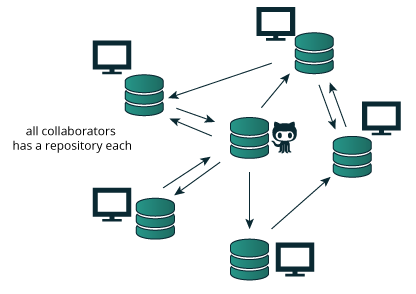
\includegraphics[width=0.6\linewidth]{images/distributed-vc}
		\end{figure}
		\tiny \hyperlink{http://thepilcrow.net/explaining-basic-concepts-git-and-github/}{http://thepilcrow.net/explaining-basic-concepts-git-and-github/} 
	\end{frame}
	\begin{frame}{Git - basic operations}
		Configuring git
		\begin{semiverbatim}
			\$ git config --global user.name "<user-name>" 
			\newline
			\$ git config --global user.email "<email-address>"
		\end{semiverbatim}
		Creating a repository
		\begin{semiverbatim}
			\$ git init <repo-name>
		\end{semiverbatim}
		Cloning a repository
		\begin{semiverbatim}
			\$ git clone <repo-url>
		\end{semiverbatim}
	\end{frame}
	\begin{frame}{Git - basic operations (cont.)}
		\begin{columns}
			\column{0.5\linewidth}
				Synchronizing changes
				\begin{semiverbatim}
					\$ git fetch
					\newline
					\$ git pull
					\newline
					\$ git push
					\newline
					\$ git merge <branch>
				\end{semiverbatim}
			\column{0.5\linewidth}
				Making changes
				\begin{semiverbatim}
					\$ git status
					\newline
					\$ git add
					\newline
					\$ git commit -m "<message>"
					\newline
					\$ git diff
				\end{semiverbatim}
		\end{columns}
	\end{frame}
	\begin{frame}{Git - data flow}
		\begin{figure}
			\centering
			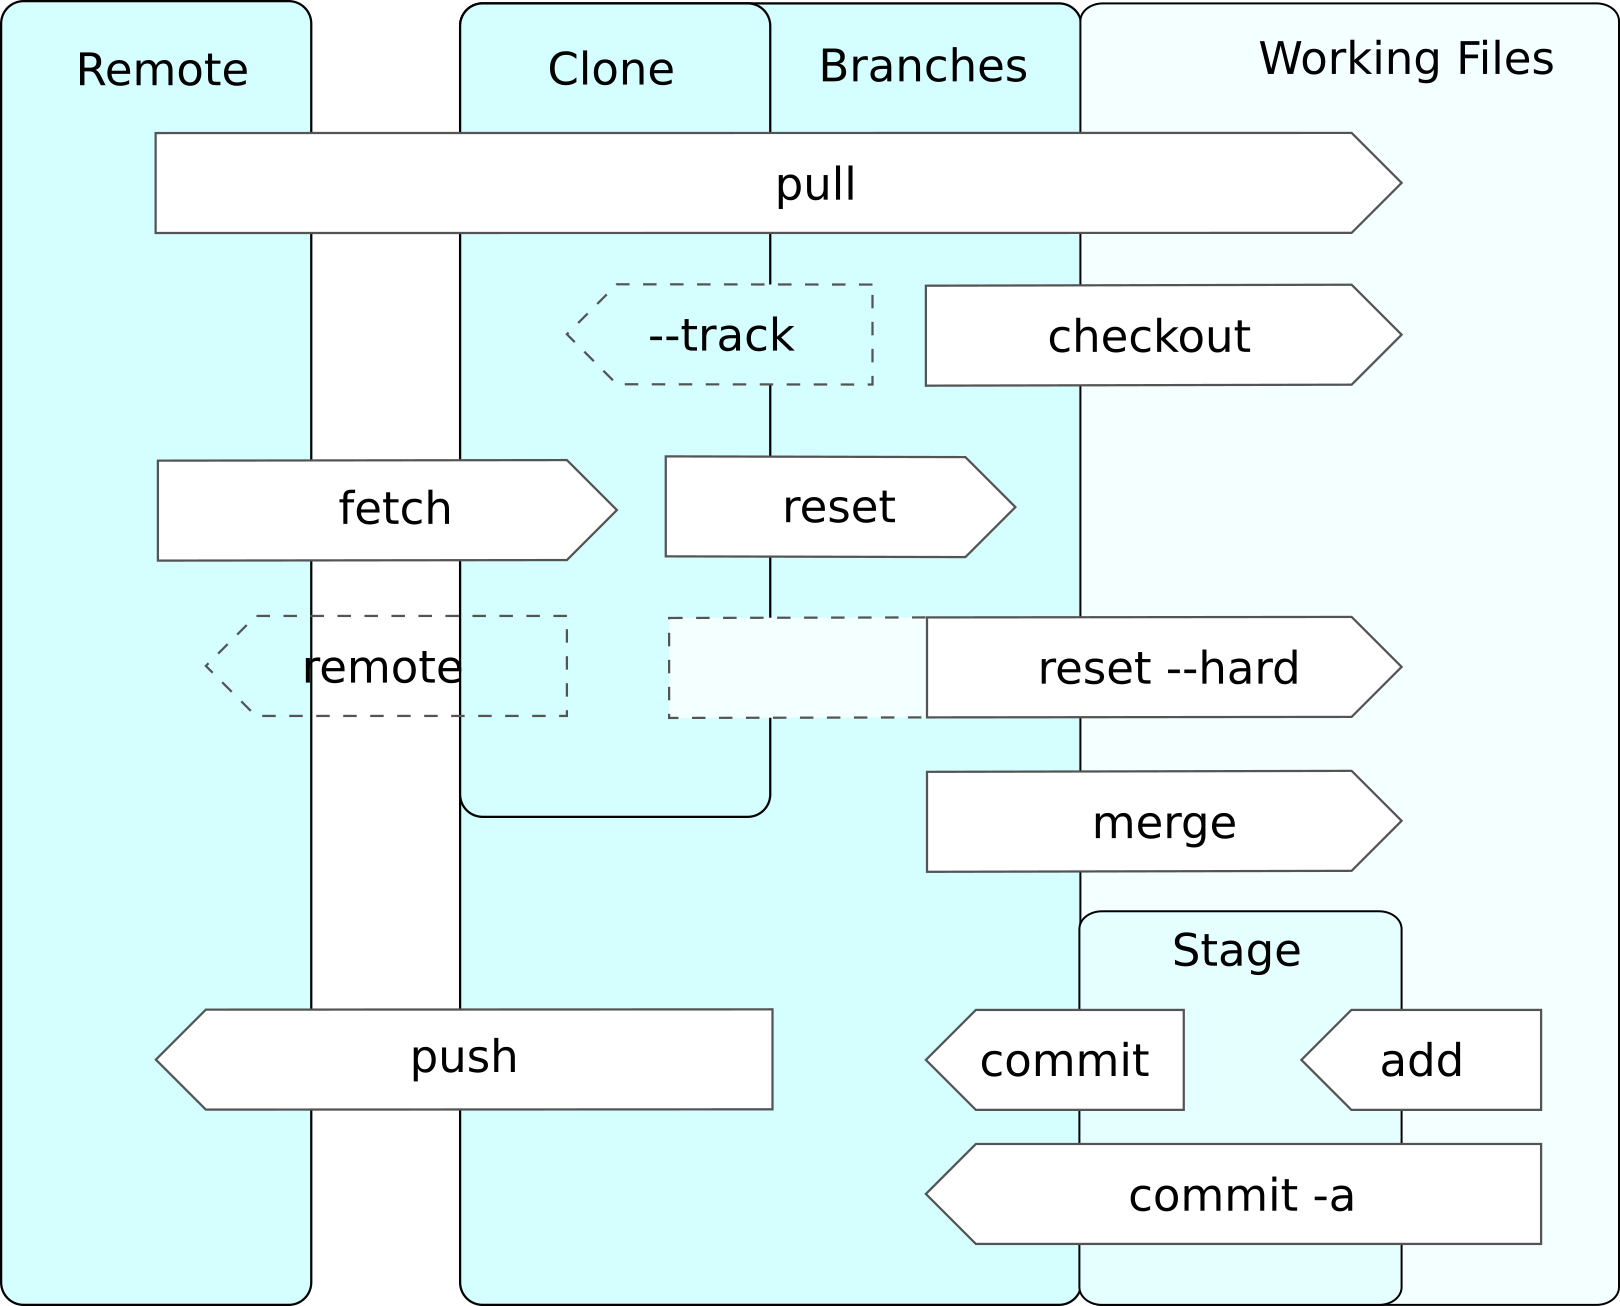
\includegraphics[width=0.5\linewidth]{images/Git_operations.png}
		\end{figure}
		\tiny \hyperlink{https://en.wikipedia.org/wiki/Git}{https://en.wikipedia.org/wiki/Git}
	\end{frame}
	\begin{frame}{Git - references}
		\Large
		\textbf{Git cheat sheet by GitHub}\\  \hyperlink{https://services.github.com/on-demand/downloads/github-git-cheat-sheet.pdf}{https://services.github.com/on-demand/downloads/github-git-cheat-sheet.pdf}
		
		\bigskip
		
		\textbf{Visual git cheat sheet}\\ \hyperlink{http://ndpsoftware.com/git-cheatsheet.html}{http://ndpsoftware.com/git-cheatsheet.html}
	\end{frame}
	
	\begin{frame}{Workflow - GitHub flow}
		\begin{enumerate}
			\item Create a branch
			\item Add commits
			\item Open a Pull Request
			\item Discuss and review your code
			\item Deploy \& test
			\item Merge
		\end{enumerate}
		 \hyperlink{https://guides.github.com/introduction/flow/}{https://guides.github.com/introduction/flow/}
	\end{frame}
	
	\section{Technologies}
	\begin{frame}{Architecture}
		\begin{figure}
			\centering
			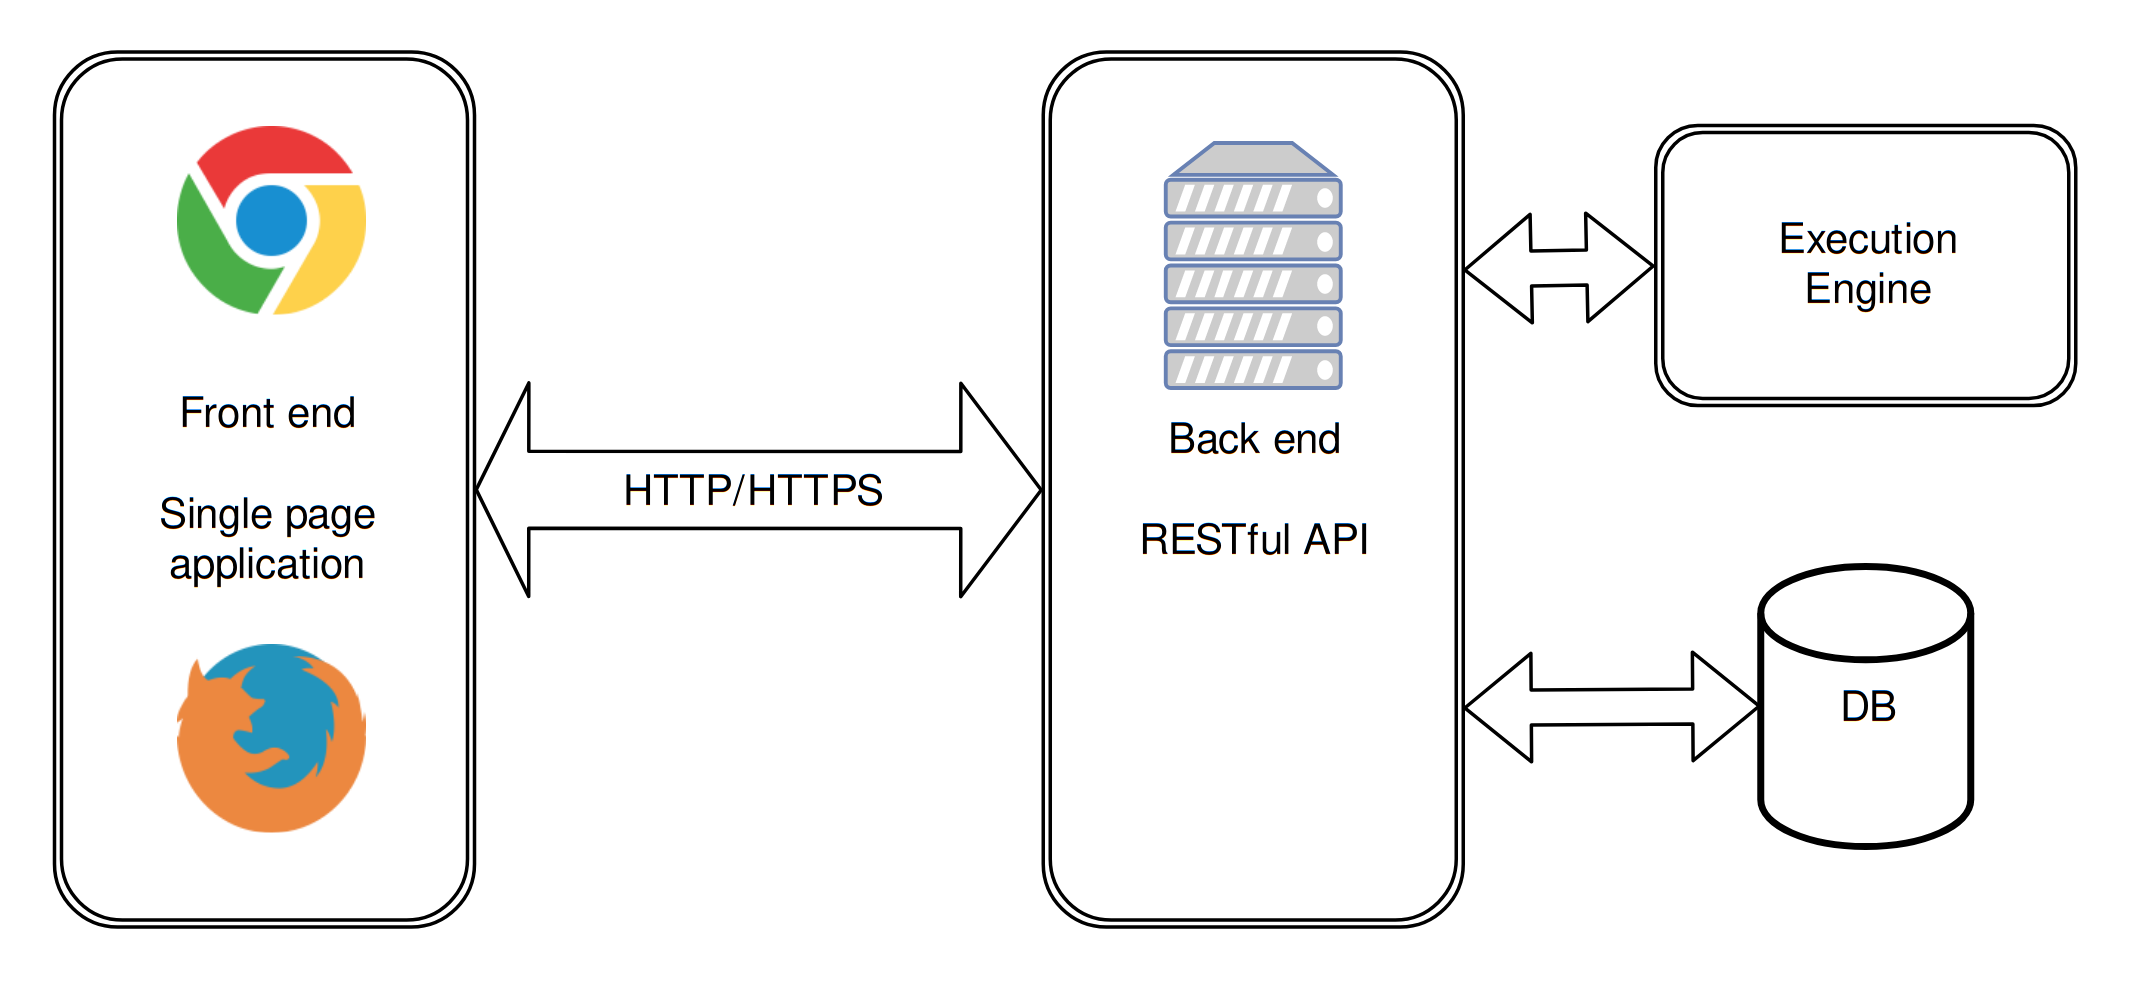
\includegraphics[width=0.8\linewidth]{images/arch}
		\end{figure}
	\end{frame}
	\begin{frame}{Docker}
	\begin{columns}
		\column{0.6\linewidth}
		\Large \textbf{Conceepts}
		\begin{itemize}
			\normalsize
			\item Docker engine
			\item docker containers
			\item dockerfile
			\item Docker SDK
		\end{itemize}
		\column{0.4\linewidth}
		\begin{figure}
			\centering
			
\includegraphics[width=1.0\linewidth]{images/dockerwhalehero}
		\end{figure}
	\end{columns}
	\tiny Image: https://www.techrepublic.com/article/how-to-run-nginx-as-a-docker-container/
	\end{frame}
	\begin{frame}{Front end \& back end}
		\begin{columns}
			\column{0.5\linewidth}
			\Large \textbf{Front end}
			\begin{itemize}
				\normalsize
				\item Angular
				\item React
				\item Vue.js
				\item etc.
			\end{itemize}
			\column{0.5\linewidth}
			\Large \textbf{Back end}
			\begin{itemize}
				\normalsize
				\item Spring Boot
				\item ASP.NET Core
				\item etc.
			\end{itemize}
		\end{columns}
	\end{frame}
	\begin{frame}{Database}
		\begin{itemize}
			\item MySQL / MariaDB
			\item PostgreSQL
			\item MongoDB
		\end{itemize}
	\end{frame}
		
	\section{Design}
	\begin{frame}{Features}
		\begin{description}
			\item[User roles] What type of user are there in this platform?
			\item[Use cases] What actions can users do in this platform?
			\item[Specifications] Are there some requirements or limitations on these use cases?
		\end{description}
	\end{frame}
	\begin{frame}{User stories}
		\large \textbf{Example: Launch a script}
		
		\normalsize
		\bigskip
		As a \textbf{script user}, I want to \textbf{launch a script}.
		\begin{enumerate}
			\item I open the scripts page
			\item I click on a script on the script list to choose it
			\item I will be redirected to a script launching page
			\item I type in the parameters
			\item I click on the launch button
			\item I will see a dialog showing the progress
			\item I see the result of the execution
		\end{enumerate}
	\end{frame}
	\begin{frame}{UI design}
		\LARGE As you have learned in OOAD Lab1.
	\end{frame}
	
	\section{Thanks}
\end{document}